\documentclass[11]{article}
\usepackage[utf8]{inputenc}
\usepackage{float}
\usepackage[pdfstartview=FitH, CJKbookmarks=true, bookmarksnumbered=true,
            bookmarksopen=true,
            colorlinks, pdfborder=001, linkcolor=red, anchorcolor=blue, citecolor=blue]{hyperref}
\usepackage{ragged2e, amsmath,  array, amsfonts}
\usepackage{tcolorbox, color}
\usepackage{caption, subcaption, graphicx}


\tcbuselibrary{theorems}

\newtcbtheorem[number within=section]{mytheo}{  }%
{colback=white!5,colframe=red!50!black,fonttitle=\bfseries}{th}

\title{Value-sensitive product (content) recommendation}
\author{Aditya Kiran }
\date{\today}


%%

\definecolor{akcolor_red}{rgb}{0.7, 0.11, 0.11}
\definecolor{akcolor_white}{rgb}{1.0, 1.0, 1.0}
\definecolor{akcolor_green}{rgb}{0.13, 0.55, 0.13}
\newcommand{\redak}[1]{{\color{akcolor_red} #1} }
\newcommand{\whiteak}[1]{{\color{akcolor_white} #1} }
\newcommand{\greenak}[1]{{\color{akcolor_green} #1} }
\newcommand{\blueak}[1]{{\color{blue} #1} }

%%%%%%%%%%%%%%%%%%%%%%%%%%%%%%%%%%%
\def\ba{\ensuremath{{\bf a}}} \def\bA{\ensuremath{{\bf A}}}
\def\bb{\ensuremath{{\bf b}}} \def\bB{\ensuremath{{\bf B}}}
\def\bc{\ensuremath{{\bf c}}} \def\bA{\ensuremath{{\bf C}}}
\def\bd{\ensuremath{{\bf d}}}\def\bD{\ensuremath{{\bf D}}}
\def\be{\ensuremath{{\bf e}}}\def\bE{\ensuremath{{\bf E}}}
\def\bF{\ensuremath{{\bf F}}}
\def\bg{\ensuremath{{\bf g}}}\def\bG{\ensuremath{{\bf G}}}
\def\bh{\ensuremath{{\bf h}}}\def\bH{\ensuremath{{\bf H}}}
\def\bi{\ensuremath{{\bf i}}}\def\bI{\ensuremath{{\bf I}}}
\def\bj{\ensuremath{{\bf j}}}\def\bJ{\ensuremath{{\bf J}}}
\def\bk{\ensuremath{{\bf k}}}\def\bK{\ensuremath{{\bf K}}}
\def\bl{\ensuremath{{\bf l}}}\def\bL{\ensuremath{{\bf L}}}
\def\bm{\ensuremath{{\bf m}}}\def\bM{\ensuremath{{\bf M}}}
\def\bn{\ensuremath{{\bf n}}}\def\bN{\ensuremath{{\bf N}}}
\def\bo{\ensuremath{{\bf o}}}\def\bO{\ensuremath{{\bf P}}}
\def\bp{\ensuremath{{\bf p}}}\def\bP{\ensuremath{{\bf P}}}
\def\bq{\ensuremath{{\bf q}}}\def\bQ{\ensuremath{{\bf Q}}}
\def\br{\ensuremath{{\bf r}}}\def\bR{\ensuremath{{\bf R}}}
\def\bs{\ensuremath{{\bf s}}}\def\bS{\ensuremath{{\bf S}}}
\def\bt{\ensuremath{{\bf t}}}\def\bT{\ensuremath{{\bf T}}}
\def\bu{\ensuremath{{\bf u}}}\def\bU{\ensuremath{{\bf U}}}
\def\bv{\ensuremath{{\bf v}}}\def\bV{\ensuremath{{\bf V}}}
\def\bw{\ensuremath{{\bf w}}}\def\bW{\ensuremath{{\bf W}}}
\def\bx{\ensuremath{{\bf x}}}\def\bX{\ensuremath{{\bf X}}}
\def\by{\ensuremath{{\bf y}}}\def\bY{\ensuremath{{\bf Y}}}
\def\bz{\ensuremath{{\bf z}}}\def\bZ{\ensuremath{{\bf Z}}}
%%%%%%%%%%%%%%%%%%%%%%%%%%%%%%%%%%%

\DeclareMathOperator{\sech}{sech}
\DeclareMathOperator{\csch}{csch}

\newcommand{\sdhd}[1]{\raggedright{\textbf{#1}} \setlength\parindent{2em}}
%%%%%%%%%%%%%%%%%%%%%%%%%%%%%%%%%%%
\newcommand{\parfrac}[2]{\frac{\partial #1}{\partial #2}}
\newcommand{\imcenter}[3]{
\begin{figure}[H]
\begin{center}
\includegraphics[#1]{#2}
\caption{#3}
\end{center}
\end{figure} }

\newcommand{\imcenterlabel}[4]{
\begin{figure}[H]
\begin{center}
\includegraphics[#1]{#2}
\caption{#3}
\end{center}
\label{#4}
\end{figure} }


\newcommand{\eqnsrightflower}[1]{
\begin{equation}
\left.
\begin{array}{lcl}
#1
\end{array}
\right\}
\end{equation}
}

\newcommand{\mincon}[2]{
\begin{equation}
\begin{aligned}\
& \underset{ #2}{\text{Minimize}}
& &   {#1} \\
\end{aligned}
\end{equation}
}


\DeclareMathOperator*{\argmin}{arg\,min}
\DeclareMathOperator*{\argmax}{arg\,max}




\newcommand{\kp}{\redak{K_p} }
\newcommand{\ki}{\greenak{K_i} }
\newcommand{\kd}{\blueak{K_d} }


%%%%%%%%%%%%%%%%%%%%%%%%%%%%%%%%%%%%%%%%%%%%%%%%%%%%%%%%%%%%
\begin{document} %JSR
\maketitle
\section{Abstract}


\section{Introduction}

\section{Formulation}
For each article $A_i$ in our database we know its 3 properties:
\begin{enumerate}

\item \textbf{$v^1_i$ is a vector of its graph-representation}:

Let $(V^1, E^1)$ be the coviewership graph. Here $V^1$ represents the set of graph-embeddings of all nodes (articles) $v^1$, and $E^1$ represents set of all edges connecting those nodes.  $d^1_{ij}$'s be the distance between $v^1_i$ and $v^1_j$. 
 
\item \textbf{$v^2_i$ is a vector of its sentence embedding}:

Let $(V^2, E^2)$ be the similarity graph. As above, $d^2_{ij}$'s be the distance between $v^2_i$ and $v^2_j$.

\item \textbf{$c_i$ is the value associated with that article}
\end{enumerate}
So, each article $A_i$ is represented by this triad $\{ v^1_i, v^2_i, c_i \}$. Although, this is a very general formulation. For the sake of simplicity, for now we will just assume that each the article is characterized by its sentence embedding and its value.

\redak{\sdhd{Problem Statement:}}

Now, the problem statement is: \\
Given that a user is reading an article $A_i$, what article must be recommended next so that we
\begin{enumerate}
\item maximize the chances of them reading more articles 
\item maximize the ad-monetary value.
\end{enumerate} 

Mathematically, given $A_i$, we seek $A_j$ such that:
\begin{align*}
 j&= \argmax_J   \phi(A_i, A_{J}) ,
\end{align*}
where $\phi$ is the utility function.

\sdhd{\redak{How do we choose the utility function?}}

Each article $A_J$ is attributed with its sentence-embedding and its value. So we need to design a utility function $\phi$ that maps its attributes to a real value:
\[ \phi: \mathbb{R}^D\times\mathbb{R}^D\times\mathbb{R}\ \to \mathbb{R} \]

\begin{itemize}
\item $\phi$ must be directly proportional to the  article's value \[ \phi(A_i, A_{J})  \propto c_J \]
\item $\phi$ must be inversely proportional to the  distance of the article $A_J$ from the current article $A_i$ \[ \phi(A_i, A_{J})  \propto \frac{1}{|d_i-d_J|} =\frac{1}{d_{iJ}} \]
\end{itemize}

Hence, we choose $$\phi(A_p, A_{q}):=\dfrac{(c_{q})^{r_1}}{(d_{pq})^{r_2}}.$$ Here $r_1$ and $r_2$ are the parameters that control the contribution of the value and the distance, on the utility term $\phi$ respectively. \\Note: The special case of $\{r_1=0, r_2=1 \}$ reduces the method back to the BAU.

\sdhd{\redak{Assumptions made:}}
\begin{enumerate}
\item The value of an article $\approx$ its $\left(\dfrac{\text{revenue}}{\text{impressions}} \right)$  from the past
\item Ignore all articles with zero revenue or impressions
\item Each article is characterized by the 512-vector Spacy embedding of its post\_title+meta\_title+summary
\end{enumerate}


\sdhd{\redak{Formulation for Infinite scroll:}} Quite often, we recommend more than just one article, either in the form of infinite-scroll or the `\textit{Next Page}' option.

So a more general form of the problem is:
Given an article $A_i$, we seek (N-1) articles $\{A_{a_1}, A_{a_2}, \cdots A_{a_{N-1}}\}$ such that:
\begin{align*}
\{a_1 \cdots a_{N-1}\} &= \argmax_{\{b_1\cdots b_{{N-1}}\}}  \sum_{k=1}^{N-1}  \gamma^{k-1} \phi(A_i, A_{b_k}),
\end{align*}
where $0<\gamma<1$ is called the discount factor.

Finally, after we know the `optimal' recommendations, we evaluate the discounted value as \[\mathcal{V}_{disc}:=\sum_{k=1}^{N-1}  \gamma^{k-1} c_{a_k} \]
We use the discounted-value instead of actual value to account for the fact that the likelihood of a user reading an article decreases with the scroll depth.

\section{Results}

\sdhd{\redak{Simulation results for infinite scroll:}}\\
We used $r_1=0.8, r_2=15, \gamma=0.09, N=6,$ and ran 30000 random simulations.
\begin{itemize}
\item We observe a lift of 41.96\% in the discounted value
\[ \left( \dfrac{  \mathcal{V}^{new}_{disc}-\mathcal{V}^{BAU}_{disc}  }{\mathcal{V}^{BAU}_{disc} } \right) \times 100  =41.96\% \]

\item Mean cosine-similarity between the recommended articles and the article being read:
\begin{itemize}
\item Purely distance-based: 0.665
\item Value-distance based: 0.658
\end{itemize}
\end{itemize}

\begin{figure}[H]
	\centering
	\begin{subfigure}[t]{0.45\textwidth}
		\centering
		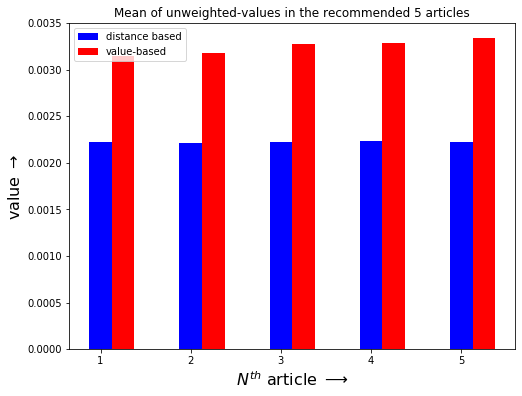
\includegraphics[width=1.1\linewidth]{images/value_abs_recomm.png} 
		\caption{Mean of unweighted-values in the recommended $(N-1)$ articles} \label{im:11}
	\end{subfigure}
	\hfill%\hspace{1.8in}
	\begin{subfigure}[t]{0.45\textwidth}
		\centering
		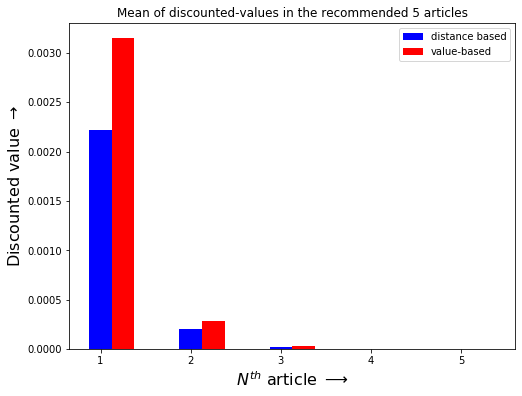
\includegraphics[width=1.1\linewidth]{images/value_weight_recomm.png}
		\caption{Mean of the discounted-values} \label{im:12}
	\end{subfigure}
	\begin{subfigure}[t]{0.49\textwidth}
		\centering
		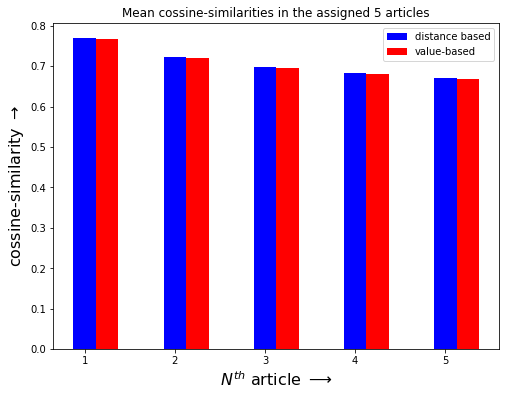
\includegraphics[width=1.0\linewidth]{images/cossim_recomm.png}
		\caption{Mean cosine-similarities} \label{im:22}
	\end{subfigure}	
	
	\caption{Conglomerated results of the recommended articles after doing the random simulations.} \label{im:33}
\end{figure}

\imcenter{width=1.1\textwidth}{images/example.png}{Example recommendations showing a lift in the value for the same set of articles.}

\section{Conclusion}
As seen from Fig. (\ref{im:22}), by achieving an almost equal cosine similarity score as the BAU, we are achieving a higher value (Fig. (\ref{im:12})) using the value-based method.

Hence we think that it is worth implementing this value-based recommendation method into a live A/B test with the BAU.


\end{document}
